\documentclass[10pt,a4paper]{exam} % turn it into a class! 
\usepackage[latin1]{inputenc}
\usepackage{amsmath}
\usepackage{amsfonts}
\usepackage{amssymb}
\usepackage{graphicx}
\usepackage{titlesec}
\usepackage{hyperref}
\usepackage{fancyeq}
\usepackage{tikz}
%\usepackage{tikz-uml}
\usepackage{mathpartir}
\usetikzlibrary{matrix,decorations.pathmorphing,shapes,arrows,backgrounds,positioning}
\usepackage{graphicx,xcolor}
\usepackage{geometry}
\usepackage{everysel}
\usepackage[normalem]{ulem}
\usepackage{natbib}

\tikzset{
  treenode/.style = {align=center, inner sep=0pt, text centered,
    font=\sffamily},
  arn_n/.style = {treenode, circle, black, font=\sffamily\bfseries, draw=black,
    fill=white, text width=1.5em},% arbre rouge noir, noeud noir
  arn_r/.style = {treenode, circle, red, draw=red, 
    text width=1.5em, very thick},% arbre rouge noir, noeud rouge
  arn_x/.style = {treenode, rectangle, draw=black,
    minimum width=0.5em, minimum height=0.5em}% arbre rouge noir, nil
}

\usepackage[sc]{mathpazo}
\linespread{1.05}         % Palatino needs more leading (space between lines)
\usepackage[T1]{fontenc}

% some format settings
% for hard-bound final submission, use:
%\setlength{\oddsidemargin}{4.6mm}     % 30 mm left margin - 1 in
% for soft-bound version and techreport, use instead:

\setlength{\oddsidemargin}{-0.4mm}    % 25 mm left margin - 1 in
\setlength{\evensidemargin}{\oddsidemargin}
\setlength{\topmargin}{-5.4mm}        % 20 mm top margin - 1 in
\setlength{\textwidth}{160mm}         % 20/25 mm right margin
\setlength{\textheight}{237mm}        % 20 mm bottom margin
\setlength{\headheight}{5mm}
\setlength{\headsep}{5mm}
\setlength{\parindent}{0mm}
\setlength{\parskip}{\medskipamount}
\renewcommand\baselinestretch{1.2} % thesis format (not needed for techreport)
% don't let large figures hijack entire pages
\renewcommand\topfraction{.9}
\renewcommand\textfraction{.1}
\renewcommand\floatpagefraction{.8}

\pagestyle{headandfoot}
%\pointsinrightmargin
%\pointname{ marks}
%\marginpointname{ marks}

\marksnotpoints 

\definecolor{campurple}{HTML}{862D91} 
\definecolor{campurpledark}{HTML}{2A185C}

\hypersetup{  
  urlcolor=campurple,
  linkcolor=campurple,
  colorlinks=true  
}

\titlelabel{\llap{\thetitle\quad}}

\newcommand {\lbrac} {\makebox[0pt]{[\kern-1ex[}}
\newcommand {\rbrac} {\makebox[0pt]{]\kern-1ex]}}
\newcommand{\denote}[1]{\lbrac~#1~\rbrac}


\def\mystrut(#1,#2){\vrule height #1pt depth #2pt width 0pt} 

\titlespacing*{\section}{0pt}{0pt}{0pt}


\begin{document}
	


\newcommand{\course}{Compiler Construction}
\newcommand{\week}{III}
\newcommand{\topics}{}

\everymath{\color{campurpledark}}
\everydisplay{\color{campurpledark}}

%\vspace{15pt}

%\begin{center}
%\emph{Complete SECTION 1 and ONE other section.}
%\end{center}

%\begin{center}
%\emph{Answer SECTION 1 and TWO other sections.}
%\end{center}

\marksnotpoints
\pointsdroppedatright
\marksnotpoints
\marginpointname{ \points}

\immediate\write18{git rev-parse --short HEAD > commit.tex}
\immediate\write18{date > date.tex}

\begin{center}
\LARGE {\textbf{\color{campurpledark} \course} }\\[-0.2cm]
\Large \color{campurpledark} Exercise \week\\
{
	\footnotesize Compiled on \input{date} using commit \input{commit}
}
\end{center}

{\color{campurple}\hrule}

\newcommand{\terminal}[1]{\texttt{\color{campurple}#1}}
\newcommand{\bl}[1]{{\color{black}#1}}

\vspace{0.5cm}

All exercises marked with (Practical) do not need to be completed in time for the supervision, but you should still do them. The previous practical exercises are prerequisites for the ones in this exercise.

In the previous exercise, we described the STG machine which serves as a target machine for non-strict functional languages, such as Haskell. However, it is not really feasible to build hardware based on this design simply to enable us to run \emph{e.g.} Haskell programs. This was attempted for \emph{e.g.} Lisp in the 80s with Lisp machines\footnote{\url{http://en.wikipedia.org/wiki/Lisp_machine}} which ultimately could not compete with other systems. In this exercise we will explore how the STG machine can be mapped to stock hardware -- \emph{e.g.} a x86 or ARM machine. Instead of dealing with the specifics of some CPU architecture, we will instead map the STG machine to C for portability. 

\begin{questions}

\section*{Implementing the STG-machine on stock hardware}
\question
\begin{parts}
	\part[4] Describe what calling conventions are and what they are used for. Illustrate your answer using an example in pseudo assembly code. \droppoints 
	\part[2] Explain the difference between calling conventions and evaluation strategies. \droppoints 
	\part[2] A compiler author is writing a code generator which targets the C language. His intention is to implement CPS so that each function from his source language is translated into a C function which pops its continuation off an argument stack and then calls the continuation at the end. For ``convenience'', he defines the following macro:
	\begin{verbatim}
	#define JUMP(x) (*x)()
	\end{verbatim}
	He then uses the macro to jump to continuations:
	\begin{verbatim}
	void foo() {
	  void* cont = *Stack--; // pop continuation off the stack
	  // code for foo
	  JUMP(&cont); // cont is the continuation
	}
	\end{verbatim}
	Explain potential pitfalls with this implementation of CPS. \droppoints 
	\part[2] The compiler author reconsiders his approach in light of your answer to the previous question and changes the signatures of all C functions to \emph{e.g.}:
	\begin{verbatim}
	void* foo();
	\end{verbatim}
	He also changes his macro to:
	\begin{verbatim}
	#define JUMP(x) return(x)
	\end{verbatim}
	Finally, he implements the following:
	\begin{verbatim}
	int main(int argc, char** argv) {
	  void* cont = &foo;
	  while(1) { cont = (*cont)(); }
	  return 0;
	}
	\end{verbatim}
	Explain why this approach is better. \droppoints 
	\part[2] If the compiler author were to choose an assembly language as the target language for his compiler, how should he implement CPS then? \droppoints 
\end{parts}
\question  Recall that configurations in the STG-machine are 6-tuples consisting of:
\begin{enumerate}
	\item the code to be executed
	\item the argument stack ($\mathit{as}$), which contains values
	\item the return stack ($\mathit{rs}$), which contains continuations
	\item the update stack ($\mathit{us}$), which contains update frames
	\item the heap ($h$), which contains closures
	\item the global environment ($\sigma$), which gives the addresses of all closures defined at top level
\end{enumerate}
How do we map these to a C program? We begin by looking at the heap. For this purpose, we will distinguish between two kinds of objects on the heap:
\begin{itemize}
	\item \emph{Head normal forms} or \emph{values} are heap objects which can not be evaluated any further, and
	\item \emph{suspensions} or \emph{thunks} are heap objects which have not yet been evaluated
\end{itemize}
Collectively, we will refer to values and thunks as \emph{closures}. Traditionally, a closure consists of a pointer to the code of a suspended computation (\emph{i.e.} just a pointer to some code), and the values of all free variables. For example, think about the Further Java exercises in which you created anonymous methods and classes. Those resulted in the creation of closures which contained copies of the variables that were captured by the anonymous methods or classes. 
\begin{center}
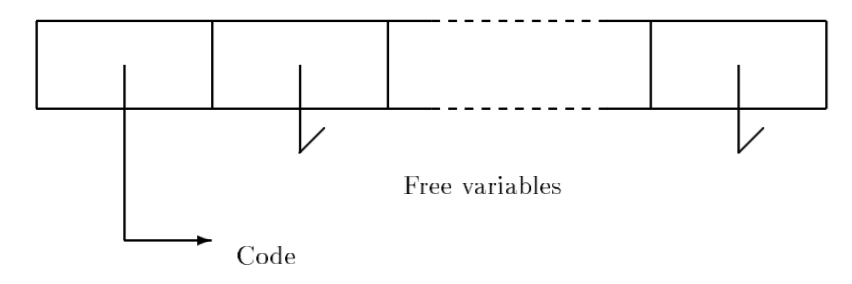
\includegraphics[scale=0.5]{closure}
\end{center}
In the STG-machine we use this representation for both, values and thunks. This corresponds to the way we represent closures in the operational semantics. \emph{I.e.} the $\mathit{Eval}~e~\rho$ code component consists of an expression $e$ (the code) and the local environment $\rho$ (the free variables). 
\begin{parts}
	\part[2] Show how you would represent STG closures in a low-level systems language, such as C, and explain your answer.  \droppoints 
	\part[4] It is possible to generate static\footnote{In this case, static means ``generated at compile-time''.} closures for all global bindings. Generate closures and function prototypes (stubs) in C for all global bindings in the following STG program.
	\begin{center}
		\begin{tabular}{lcl}
			\texttt{nil} & \texttt{=} & \texttt{\{\} \textbackslash n \{\} -> Nil \{\}}\\
			\texttt{succ} & \texttt{=} & \texttt{\{\} \textbackslash n \{x\} -> +\# \{x, 1\#\}}\\
			\texttt{list} & \texttt{=} & \texttt{\{\} \textbackslash n \{\} -> Cons \{5\#, nil\}}\\
			\texttt{map} & \texttt{=} & \texttt{\{\} \textbackslash n \{f,xs\} ->} \\
			&   & \quad \texttt{case xs \{\}  of} \\
			&   & \quad \begin{tabular}[t]{lcl}
				\texttt{Nil \{\}} & \texttt{->} & \begin{tabular}{l}
					\texttt{Nil \{\}}
				\end{tabular}  \\
				\texttt{Cons \{y,ys\}} & \texttt{->} & \begin{tabular}[t]{llcl}
					\texttt{let} & \texttt{fy} & \texttt{=} & \texttt{\{f,y\} \textbackslash n \{\} -> f \{y\}} \\
					& \texttt{mfy} & \texttt{=} & \texttt{\{f,ys\} \textbackslash n \{\} -> map \{f,ys\}} \\
					\multicolumn{4}{l}{\texttt{in Cons \{fy,mfy\}}}
				\end{tabular}
			\end{tabular} \\
			\texttt{main} & \texttt{=} & \texttt{\{\} \textbackslash n \{\} -> map \{succ, list\}}
		\end{tabular}
	\end{center} 
	For example, the C function corresponding to $\texttt{nil}$ may look like this:
	\begin{verbatim}
	void* nil_code() {
	  // do nothing yet
	  JUMP(NULL); // to make the compiler happy for now
	}
	\end{verbatim} \droppoints 
	\part[2] Explain why there is no need to implement the global environment $\sigma$ when mapping the STG machine to C. \droppoints 
	\part[1] Closures for local bindings must be allocated dynamically at runtime because we cannot predict what their free variables will be. For this purpose, we require a heap that we can allocate memory on. Do not worry about freeing memory. Show how you would implement this in C. \droppoints 
	\part[1] How would you implement a test for whether there is free space on the heap? \droppoints 
	\part[3] Suppose that a local binding $\texttt{fy}$ has a corresponding C function named \texttt{fy\_code} which captures two free variables. Show how you would allocate space on the heap for a corresponding closure and how you would initialise it, assuming that pointers to the closures for the two free variables are available in local variables named $\texttt{f}$ and $\texttt{y}$. \droppoints 
\end{parts}
\question
\begin{parts}
	\part[1] It is possible to implement all three stacks ($\mathit{as}$, $\mathit{rs}$, and $\mathit{us}$) using one concrete stack and, for simplicity, that's what we will do for now. Traditionally, stacks grow from higher memory addresses to lower memory addresses. Why? \droppoints 
	\part[3] Show how you would implement a stack in C, including sample code to push and pop items. \droppoints 
	\part[2] The process of evaluating (``entering'') a closure involves jumping to the memory address indicated by the code pointer of a closure and pushing any arguments onto the stack. How would you ensure that the code component of the closure can find its free variables? How would you address the argument? \droppoints  
	\part[4] Explain what we mean by ``boxed'' and ``unboxed'' values. Give an example of both in the STG language. \droppoints 
	\part[6] In order to evaluate a case expression whose expression $e$ evaluates to an integer literal, we need to push the address of a continuation $k$ onto the return stack, then enter the closure representing $e$. By convention, we will say that an expression which evaluates to an integer literal, stores its result in a special register (which, for portability, we can represent in C using a global variable) before invoking $k$. The continuation $k$ then examines the value stored in this register and proceeds accordingly. Translate the following to C:
	\begin{center}
		\begin{tabular}{lcl}
			\texttt{zero} & \texttt{=} & \texttt{\{\} \textbackslash n \{\} -> 0\#}\\
			\texttt{not} & \texttt{=} & \texttt{\{\} \textbackslash n \{b\} ->} \\
				&   & \quad \texttt{case b \{\}  of} \\
				&   & \quad \begin{tabular}[t]{lcl}
					\texttt{0\#} & \texttt{->} & \begin{tabular}{l}
						\texttt{1\#}
					\end{tabular}  \\
					\texttt{default} & \texttt{->} & \begin{tabular}{l}
							\texttt{0\#}
						\end{tabular}
					\end{tabular} \\
			\texttt{main} & \texttt{=} & \texttt{\{\} \textbackslash n \{\} -> not \{zero\}}
		\end{tabular}
	\end{center} \droppoints 
	\part[6] For case expressions which operate on algebraic data types, we use a different approach. Instead of pushing the address of a continuation onto the stack, we push the address of a \emph{return vector}. The return vector is an array of memory addresses pointing to different continuations, one for each constructor in the data type. An expression which evaluates to a constructor application will expect such a return vector on the stack and chooses the element corresponding to the constructor. For example, consider the following type in ML:
	\begin{displaymath}
	\mathbf{datatype}~'a~\mathit{list} = \mathit{Nil} \mid \mathit{Cons}~\mathbf{of}~'a \times ('a~\mathit{list})
	\end{displaymath}
	This type has two constructors. A return vector for this type would therefore contain two entries. The $\texttt{Nil}$ constructor will select the first entry (at offset 0) and jump to it. The $\texttt{Cons}$ constructor will allocate a closure on the heap and store its arguments in the free variable fields, then select the second entry (at offset 1) and jump to it. Translate the following to C:
	\begin{center}
		\begin{tabular}{lcl}
			\texttt{nil} & \texttt{=} & \texttt{\{\} \textbackslash n \{\} -> Nil \{\}}\\
			\texttt{null} & \texttt{=} & \texttt{\{\} \textbackslash n \{xs\} ->} \\
			&   & \quad \texttt{case xs \{\}  of} \\
			&   & \quad \begin{tabular}[t]{lcl}
				\texttt{Nil \{\}} & \texttt{->} & \begin{tabular}{l}
					\texttt{True \{\}}
				\end{tabular}  \\
				\texttt{Cons \{y,ys\}} & \texttt{->} & \begin{tabular}{l}
					\texttt{False \{\}}
				\end{tabular}
			\end{tabular} \\
			\texttt{main} & \texttt{=} & \texttt{\{\} \textbackslash n \{\} -> null \{nil\}}
		\end{tabular}
	\end{center} \droppoints 
\end{parts}
\question 
\begin{parts}
	\part[4] STG (as described in the original paper) uses the Copying Collection technique for garbage collection. Briefly explain how this works in general. \droppoints 
	\part[2] Copying Collection requires two heaps. How would you implement them space-efficiently? \droppoints 
	\part[2] Copying memory from one heap to another is a slow process. Explain one garbage collection technique which could reduce the amount of memory that has to be copied. \droppoints 
\end{parts}
\end{questions}
\end{document}
